\chapter{Projekte}
FreeQDA arbeitet in so genannten Projekten. Innerhalb eines Projektes können verschiedene Texte und Codes angelegt, gespeichert, verwaltet und %
bearbeitet werden.


\section{Ein neues Projekt beginnen}
\begin{wrapfigure}[9]{l}{0.2\textwidth}
 \vspace{-28pt}
 \begin{center}
    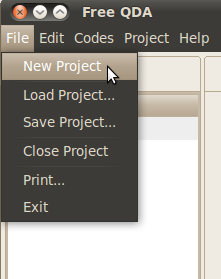
\includegraphics[width=0.18\textwidth]{img/newproject}
  \end{center}
 
%  \caption{Bereich von 2 Standard\-abweich\-ungen}
%  \label{fig:normal3}
  \vspace{12pt}
\end{wrapfigure}
Klicken Sie im Programm-Menü auf \texttt{File => New Project}. Es öffnet sich ein neues Fenster, in welchem Sie gebeten werden, den %
Namen des neuen Projektes einzugeben (siehe Abbildung \ref{fig:newproject}). Geben Sie einen Namen ein (z.B. ``Forschungsprojekt A123'') %
und klicken Sie anschließend auf \texttt{Finish}. Das neues Projekt wird hierdurch erstellt. 

Alle Projekte werden standardmäßig im Programmordner \texttt{FreeQDA/FQDAWorkspace} ab\-ge\-speichert. %In unserem Beispiel 
Jedes Projekt besitzt hier wiederum einen eigenen \textit{Projektordner} (in diesem Beispiel \texttt{Forschungs\-projekt A123}), welcher alle Dateien und Codes %
des Projekts enthält. Die eigentliche Projekt\-hauptdatei liegt auch in diesem Ordner und heisst immer \texttt{project.fqd} (siehe %
Abbildung \ref{fig:projektdatei}).
% 
\begin{figure}[!hbt]
\begin{minipage}[!hb!]{0.5\textwidth}
	\centering
	 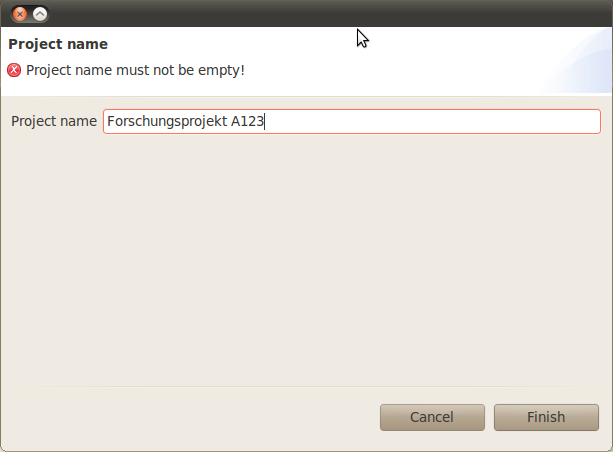
\includegraphics[width=\textwidth]{img/NewProject}
	\caption{Starten Sie ein neues Projekt}
	\label{fig:newproject}
\end{minipage}
\hfill
\begin{minipage}[!hb!]{0.5\textwidth}
	\centering
	 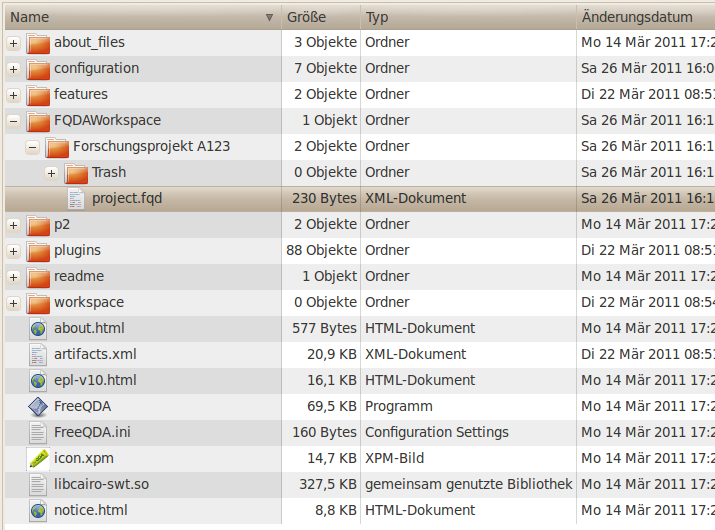
\includegraphics[width=\textwidth]{img/ProjektFile}
	\caption{Projektordner und -datei}
	\label{fig:projektdatei}
\end{minipage}
\end{figure}


\section {Ein Projekt laden}
\begin{wrapfigure}[9]{l}{0.2\textwidth}
 \vspace{-28pt}
 \begin{center}
    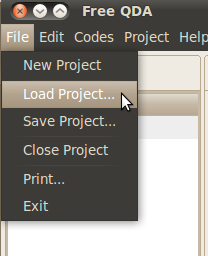
\includegraphics[width=0.18\textwidth]{img/loadproject}
  \end{center}
 
%  \caption{Bereich von 2 Standard\-abweich\-ungen}
%  \label{fig:normal3}
  \vspace{12pt}
\end{wrapfigure}
Um ein bereits vorhandenes Projekt zu laden, klicken Sie im Programm-Menü auf \texttt{File => Load Project}. Es öffnet sich ein %
Dateidialog, in welchem Sie gebeten werden, die gewünschte Projektdatei auszuwählen. Navigieren Sie zunächst in den Ordner %
\texttt{FQDAWorkspace}. Hier werden Ihnen alle vorhandenen Projektordner aufgelistet. Klicken Sie nun doppelt auf den gewünschten Ordner %
und wählen Sie die Projektdatei \texttt{project.fqd} aus. Bestätigen Sie durch einen Klick auf den \texttt{OK} Button Ihre Auswahl. %
Das Projekt wird nun geladen.


